\documentclass[0pt]{esannV2}
\usepackage{graphicx}
\usepackage{amsmath,amsfonts,amssymb,amsthm}
\usepackage[latin1]{inputenc}
\usepackage{amssymb,amsmath,array}


%***********************************************************************
% !!!! IMPORTANT NOTICE ON TEXT MARGINS !!!!!
%***********************************************************************
%
% Please avoid using DVI2PDF or PS2PDF converters: some undesired
% shifting/scaling may occur when using these programs
% It is strongly recommended to use the DVIPS converters, and to submit
% PS file. You may submit a PDF file if and only if you use ADOBE ACROBAT
% to convert your PS file to PDF.
%
% Check that you have set the paper size to A4 (and NOT to letter) in your
% dvi2ps converter, in Adobe Acrobat if you use it, and in any printer driver
% that you could use.  You also have to disable the 'scale to fit paper' option
% of your printer driver.
%
% In any case, please check carefully that the final size of the top and
% bottom margins is 5.2 cm and of the left and right margins is 4.4 cm.
% It is your responsibility to verify this important requirement.  If these margin requirements and not fulfilled at the end of your file generation process, please use the following commands to correct them.  Otherwise, please do not modify these commands.
%
\voffset 0 cm \hoffset 0 cm \addtolength{\textwidth}{0cm}
\addtolength{\textheight}{0cm}\addtolength{\leftmargin}{0cm}

%***********************************************************************
% !!!! USE OF THE esannV2 LaTeX STYLE FILE !!!!!
%***********************************************************************
%
% Some commands are inserted in the following .tex example file.  Therefore to
% set up your ESANN submission, please use this file and modify it to insert
% your text, rather than staring from a blank .tex file.  In this way, you will
% have the commands inserted in the right place.

\begin{document}
%style file for ESANN manuscripts
\title{Procesamiento de texto manuscrito usando conjuntos de clasificadores}

%***********************************************************************
% AUTHORS INFORMATION AREA
%***********************************************************************
\author{
Emilio Samuel Aced Fuentes \\
Roberto Alcober Couso \\
Arturo Bl\'azquez P\'erez \\
Nicol\'as Trejo Moya \\
}
%***********************************************************************
% END OF AUTHORS INFORMATION AREA
%***********************************************************************

\maketitle

\section{Introducci\'on}
En este proyecto vamos a clasificar im\'agenes de letras manuscritas intentando predecir de forma correcta el s\'imbolo que representan.
En nuestro primer contacto con las im\'genes, las modificaremos con la biblioteca skimage para limpiar el fondo de las manchas e impurezas del papel y cerrar los trazos que no hallan sido terminados con el objetivo de conseguir una mejor clasificaci\'on.



\section{An\'alisis de los datos}
En el dataset provisto, est\'an representadaslas 10 primeras letras del alfabeto(A-J), por tanto 10 clases las cuales hemos etiquetado en nuestra base de datos etiquetadas de 0 a 10 respectivamente.

\begin{figure}[htbp]
\centering
    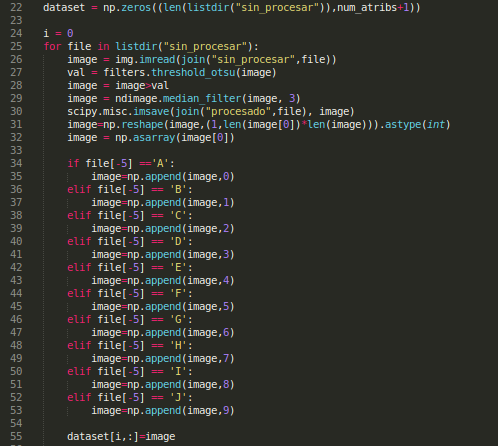
\includegraphics[width=0.8\textwidth,natwidth=906,natheight=600]{./representacion.png}
    \caption{Representaci\'on}
\end{figure}


\begin{flushleft}
Como podemos ver a continuaci\'on, hay 132 ejemplos en imagenes de 150x206 pixels generando un total de 30900 atributos en total por cada ejemplo, durante nuestro análisis veremos formas de reducir este n\'umero con el objetivo de aumentar el rendimiento y precisi\'on de nuestra clasificaci\'on. Como podemos ver en la captura de pantalla no parece haber missing values dado que hay 13200 ejemplos y hay 132 ejemplos de cada letra.
\end{flushleft}

\begin{figure}[htbp]
\centering
    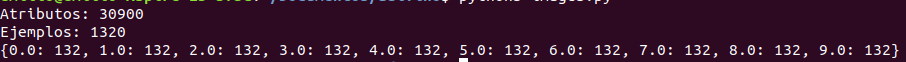
\includegraphics[width=0.8\textwidth,natwidth=906,natheight=62]{./dataset.jpg}
\caption{The Universe}
\end{figure}


\section{Atributos}
Nuestra primera aproximaci\'on a los atributos fue coger la imagen de la letra y transformarla a un array de numpy con la funci\'on img.imread(Nombre del fichero), tras esto aplicar filters.threshold\_otsu() que nos transformaba de forma autom\'atica  la imagen a blanco y negro y, por \'ultimo aplicar un filtro de mediana para eliminar las impurezas.(Ver Fig 1)


\section{Modelos}
Inicialmente pensamos que un buen candidato a clasificar nuestro conjunto de datos fue el algoritmo de Random Forest de scikit learn con 100 clasificadores de profundidad 2 y el resto de parametros por defecto, lo entrenamos con el primer 90\% de los datos y lo probamos con el 10\% restante, sin embargo, los resultados fueron bastante mediocres, un 60\% de porcentaje de acierto, por lo que probamos a aumentar la profundidad de los arboles de decisi\'on a 4, lo que mejor\'o la clasificaci\'on hasta el 75\% lo cual es bastante mejor.

\section{Typesetting an ESANN document using \LaTeX}

This is a sample file. Please use this file to correctly typeset a
submission to the ESANN conference. The associated pdf file will
help you to have an idea of what your paper should look like.

\subsection{Page format and margins}
Please avoid using DVI2PDF or PS2PDF converters: some undesired
shifting/scaling may occur when using these programs
It is strongly recommended to use the DVIPS converters, and to submit
PS file. You may submit a PDF file if and only if you use ADOBE ACROBAT
to convert your PS file to PDF.
%
Check that you have set the paper size to A4 (and NOT to letter) in your
dvi2ps converter, in Adobe Acrobat if you use it, and in any printer driver
that you could use.  You also have to disable the 'scale to fit paper' option
of your printer driver.
%
In any case, please check carefully that the final size of the top and
bottom margins is 5.2 cm and of the left and right margins is 4.4 cm.
%t is your responsibility to verify this important requirement.  If these margin requirements and not fulfilled at the end of your file generation process, please use the commands at the beginning of the ESANNV2.tex file to correct them.  Otherwise, please do not modify these commands.


\subsection{Additional packages and functions}

Update the sample file according to your text. You can add
packages or declare new \LaTeX\ functions if and only if there is no conflict between your packages and the esannV2.cls style file.

\subsection{Style information}

\subsubsection{Page numbers}
Please do not add page numbers to this style; page numbers will be added by the publisher.
\subsubsection{Page headings}
Do not add headings to your document.
\subsection{Mathematics}
You may include additional packages for typesetting
algorithms, mathematical formula or to define new operators and environments
if and only if there is no conflict with the esannV2.cls
file.

It is recommended to avoid the numbering of equations when not
necessary. When dealing with equation arrays, it could be
necessary to label several (in)equalities. You can do it using the
`$\backslash$stackrel' operator (see the ESANNV2.tex source file);
example:

\begin{eqnarray}
c&=&|d|+|e|\nonumber\\
&\stackrel{\text{(a)}}{=}&d+e\nonumber\\
&\stackrel{\text{(b)}}{\geq}&\sqrt{f}\enspace,
\end{eqnarray}
\noindent where the equality (a) results from the fact that both
$d$ and $e$ are positive while (b) comes from the definition of
$f$.

\subsection{Tables and figures}


Table \ref{Tab:AgeWeight} shows an example of table.

\begin{table}[h!]
  \centering
  \begin{tabular}{|c|c|c|}
    \hline
    ID & age & weight \\
    \hline
    1& 15 & 65 \\
    2& 24 & 74\\
    3& 18 & 69 \\
    4& 32 & 78 \\
    \hline
  \end{tabular}
  \caption{Age and weight of people.}\label{Tab:AgeWeight}
\end{table}

\section{Citation}
This ESANNV2.tex file defines how to insert references, both for
BiBTeX and non-BiBTeX users.  Please read the instructions in this
file.

% ****************************************************************************
% BIBLIOGRAPHY AREA
% ****************************************************************************

\begin{footnotesize}

% IF YOU DO NOT USE BIBTEX, USE THE FOLLOWING SAMPLE SCHEME FOR THE REFERENCES
% ----------------------------------------------------------------------------
\begin{thebibliography}{99}

% For books
\bibitem{Haykin_book} S. Haykin, editor. \emph{Unsupervised Adaptive Filtering vol.1 : Blind Source Separation}, John Willey ans Sons, New York, 2000.

% For articles
\bibitem{DelfosseLoubaton_article}N. Delfosse and P. Loubaton, Adaptibe blind separation of sources: A deflation
approach, \emph{Signal Processing}, 45:59-83, Elsevier, 1995.

% For paper in proceedings published as serie books (LNCS,...)
\bibitem{CrucCichAmari_bookproceedings} S. Cruces, A. Cichocki and S. Amari, The minimum entropy and cumulants based contrast functions for blind source extraction. In J. Mira and A. Prieto, editors, proceedings of the 6$^{th}$ \emph{international workshop on artificial neural networks} ({IWANN} 2001), Lecture Notes in Computer Science 2085, pages 786-793,
Springer-Verlag, 2001.

% For paper in conference proceedings
\bibitem{VrinsArchambeau_proceedings} F. Vrins, C. Archambeau and M. Verleysen, Towards a local separation performances estimator using common ICA contrast functions? In M. Verleysen, editor, \emph{proceedings of the $12^{th}$
European Symposium on Artificial Neural Networks} ({ESANN} 2004),
d-side pub., pages 211-216, April 28-30, Bruges (Belgium), 2004.

% For Technical Report
\bibitem{Stone_TechRep} J. V. Stone and J. Porrill, Undercomplete independent component analysis for signal separation and dimension
reduction. Technical Report, Psychology Department, Sheffield
University, Sheffield, S10 2UR, England, October 1997.
\end{thebibliography}
% ----------------------------------------------------------------------------

% IF YOU USE BIBTEX,
% - DELETE THE TEXT BETWEEN THE TWO ABOVE DASHED LINES
% - UNCOMMENT THE NEXT TWO LINES AND REPLACE 'Name_Of_Your_BibFile'

%\bibliographystyle{unsrt}
%\bibliography{Name_Of_Your_BibFile}

\end{footnotesize}

% ****************************************************************************
% END OF BIBLIOGRAPHY AREA
% ****************************************************************************

\end{document}
